\documentclass{article}
\usepackage{a4wide}
\usepackage{norsk}
\usepackage{amsmath}
\usepackage{amssymb}
\usepackage{dsfont}
%\usepackage[dvips]{epsfig}
%\usepackage{graphicx}
\usepackage{fancyhdr}
\usepackage{listings}
\usepackage{nomencl}
\usepackage[pdftex]{graphicx}

\pagestyle{fancy}
\lhead{\footnotesize \parbox{11cm}{Andreas Johann H\"ormer (753179)}}
\rhead{\footnotesize {Laboratory 1}}
\chead{\footnotesize {TTT4170}}

\title{Report Room acoustics (Lab 1)}
\author{Andreas Johann H\"ormer}
\date{14.02.2014}

\begin{document}

\maketitle
%\\[5cm]
\begin{center}
TTT4170 Audio Technology\\[3cm]
Lab group:
\begin{itemize}
\item Andreas Johann H\"ormer
\item Milan Stojkovic
\item y\\[3cm]
\end{itemize}
Report delivered: 27.02.2014\\[6cm]
FACULTY OF INFORMATION TECHNOLOGY, MATHEMATICS AND ELECTRICAL ENGINEERING\\
NORWEGIAN UNIVERSITY OF SCIENCE AND TECHNOLOGY
\end{center}

\tableofcontents

\newpage
\section{Summary}

\newpage
\section{Introduction}


\newpage
\section{Measurements}
\subsection{Equipment}
\subsection{Reverbation time}
\subsubsection{Method}
\begin{table}
\begin{center}
\begin{tabular}{|c c|}
\hline
\includegraphics[width=6cm,keepaspectratio=true]{frontpic} & 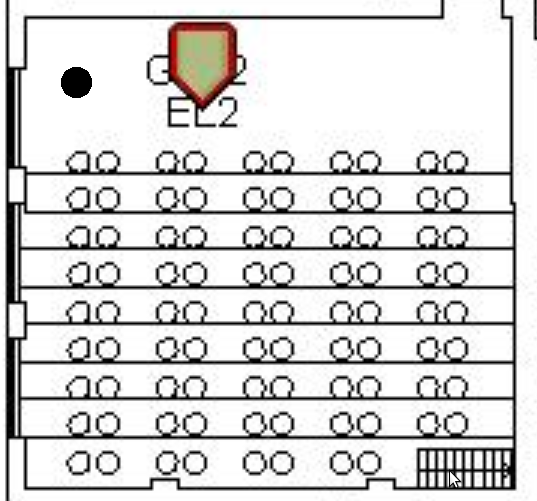
\includegraphics[width=5cm,keepaspectratio=true]{front}\\
\multicolumn{2}{|c|}{measurement in the left front corner}\\
\hline
\includegraphics[width=6cm,keepaspectratio=true]{middlepic} & 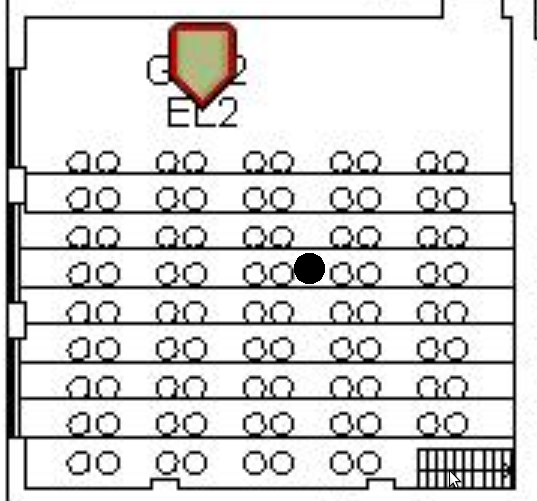
\includegraphics[width=5cm,keepaspectratio=true]{middle}\\
\multicolumn{2}{|c|}{measurement in the middle of the room}\\
\hline
\includegraphics[width=6cm,keepaspectratio=true]{backpic} & 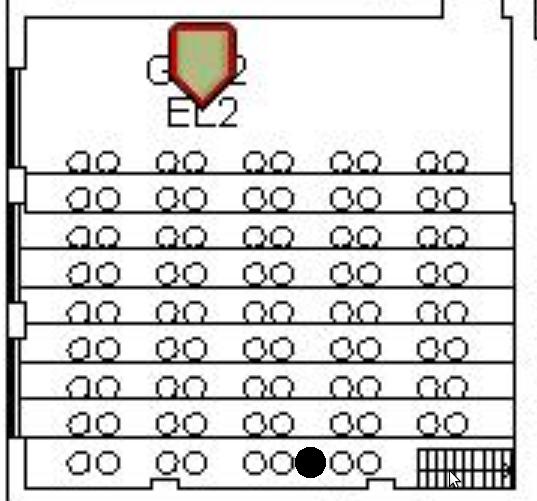
\includegraphics[width=5cm,keepaspectratio=true]{back}\\
\multicolumn{2}{|c|}{measurement at the backside}\\
\hline
\end{tabular}
\caption{microphone positions}
\label{tab:revmeasure}
\end{center}
\end{table}
\subsubsection{Results}
\begin{figure}[htbp]
\begin{center}
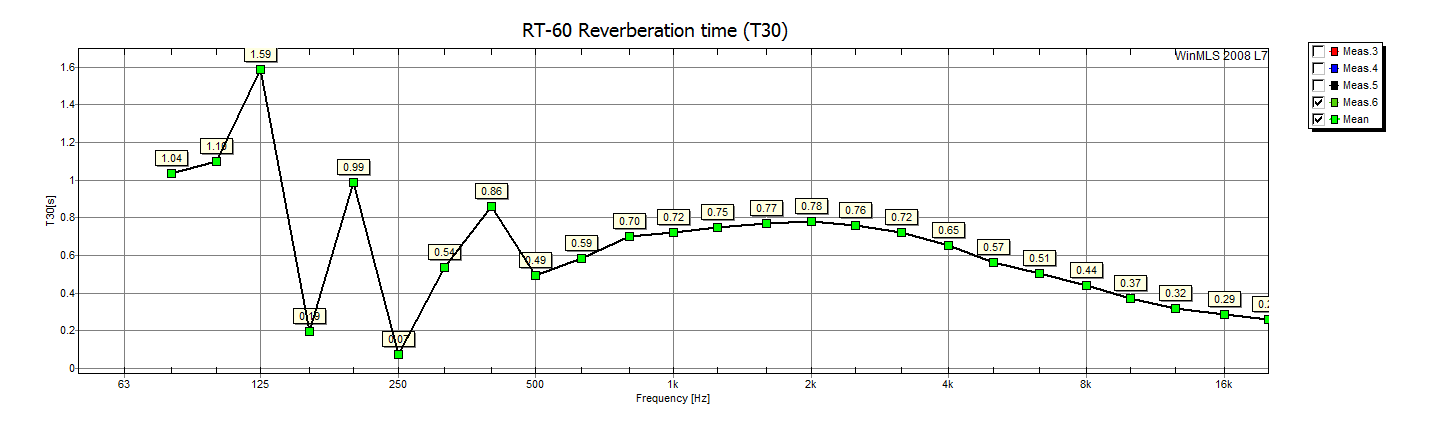
\includegraphics[width=15cm,keepaspectratio=true]{reverbationfront}
\caption{reverbation time in the front position}
\label{fig:reverbationfront}
\end{center}
\end{figure}
\begin{figure}[htbp]
\begin{center}
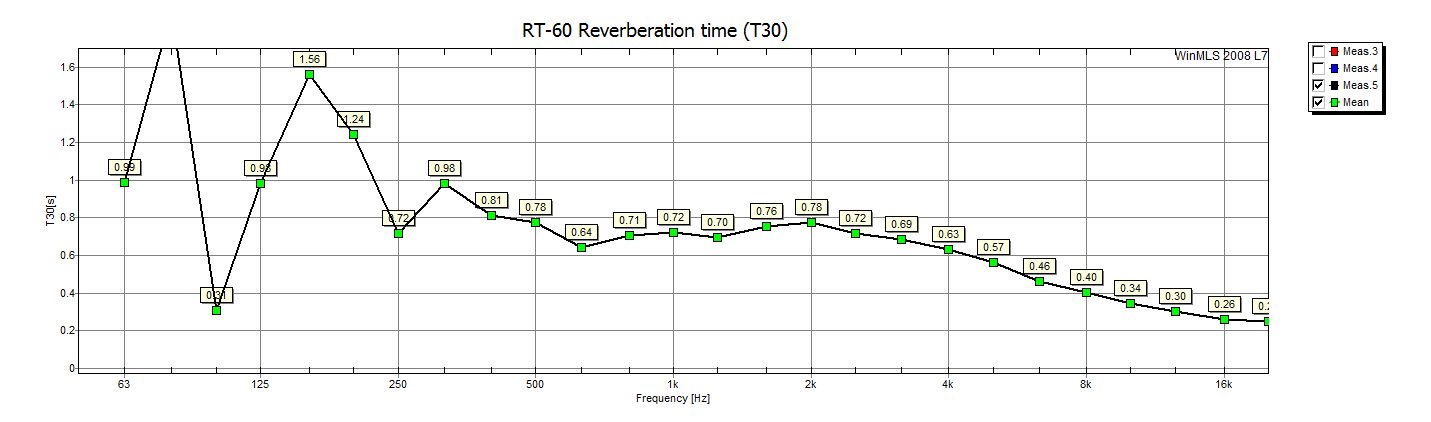
\includegraphics[width=15cm,keepaspectratio=true]{reverbationmiddle}
\caption{reverbation time in the middle position}
\label{fig:reverbationmiddle}
\end{center}
\end{figure}
\begin{figure}[htbp]
\begin{center}
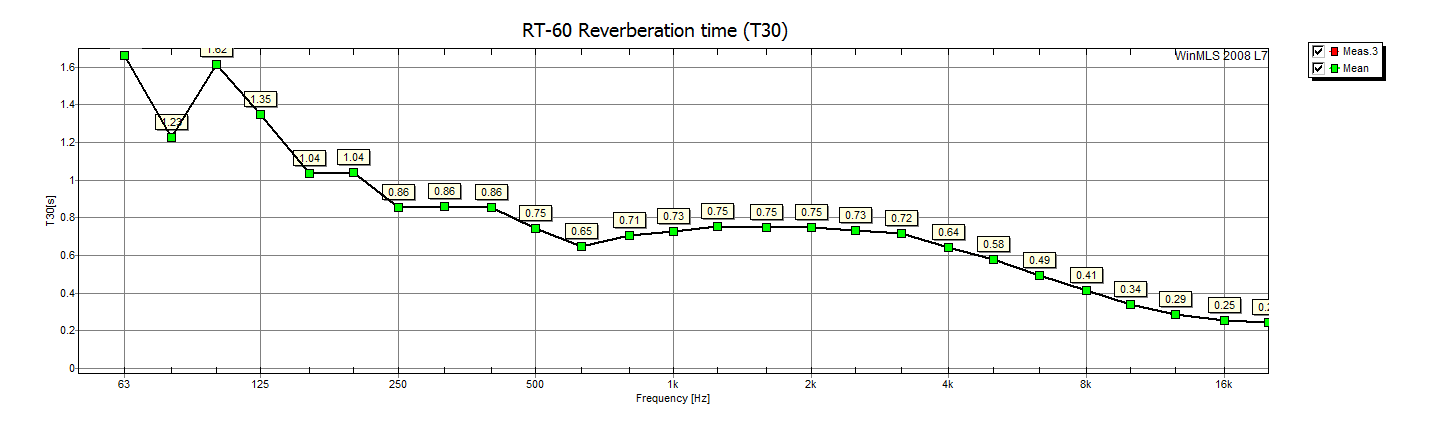
\includegraphics[width=15cm,keepaspectratio=true]{reverbationback}
\caption{reverbation time in the back position}
\label{fig:reverbationback}
\end{center}
\end{figure}
\subsection{Sound pressure level}
\subsubsection{Method}
\subsubsection{Results}

\newpage
\section{Calculations}

\newpage
\section{Conclusion}

\newpage
\section{Appendix}

\newpage
\section{References}
	
\subsection{b}
\begin{table}
\begin{center}
\begin{tabular}{|c||c|c|c||c|}
\hline
octave band & front & middle & back & average	\\
$Hz$		&	$s$	&	$s$		&	$s$		&	$s$		\\
\hline
\hline
125			& 1.34	&	0.98	&	1.58	&	1.3		\\
\hline
250			& 0.86	&	0.72	&	0.07	&	0.55	\\
\hline
500			& 0.75	& 	0.78	&	0.49	&	0.67	\\
\hline
1k			& 0.73	&	0.72	&	0.72	&	0.72	\\
\hline
2k			& 0.75	&	0.78	&	0.78	&	0.77	\\
\hline
4k			& 0.64	&	0.63	&	0.65	& 	0.64	\\
\hline


\end{tabular}
\caption{$T_{60}$ measurements and average}
\label{tab:Tmeasurements}
\end{center}
\end{table}
\subsubsection{calculations}

\subsection{d}
\subsubsection{calculations}
$$\bar{\alpha_{125}}=\frac{0.161\cdot 367m^3}{1.3s\cdot 344m^2}=0.132$$
$$\bar{\alpha_{250}}=\frac{0.161\cdot 367m^3}{0.55s\cdot 344m^2}=0.312$$
$$\bar{\alpha_{500}}=\frac{0.161\cdot 367m^3}{0.67s\cdot 344m^2}=0.256$$
$$\bar{\alpha_{1k}}=\frac{0.161\cdot 367m^3}{0.72s\cdot 344m^2}=0.239$$
$$\bar{\alpha_{2k}}=\frac{0.161\cdot 367m^3}{0.77s\cdot 344m^2}=0.223$$
$$\bar{\alpha_{4k}}=\frac{0.161\cdot 367m^3}{0.64s\cdot 344m^2}=0.268$$
\subsection{e}
$$\alpha_{1,125}=\frac{344m^2\cdot 0.132-0.7\cdot 66.75m^2}{277.25m^2}=-0.004$$
The absorbtion factor is negative which means that the chair absorption factor is overestimated. Due to the fact that absorbtion decreases with lower frequencies the absorption factor is lower at low frequencies.  An factor of $\alpha=0.4$ for a frequency of $f=125Hz$ was assumed and the resulting absorbtion factor increases to
 $$\alpha_{1,125}=\frac{344m^2\cdot 0.132-0.4\cdot 66.75m^2}{277.25m^2}=-0.067$$
All other calculations are done with an assumed absorbtion factor of $\alpha_{chair}=0.7$.
 $$\alpha_{1,250}=\frac{344m^2\cdot 0.312-0.7\cdot 66.75m^2}{277.25m^2}=0.219$$
 $$\alpha_{1,500}=\frac{344m^2\cdot 0.256-0.7\cdot 66.75m^2}{277.25m^2}=0.149$$
 $$\alpha_{1,1k}=\frac{344m^2\cdot 0.239-0.7\cdot 66.75m^2}{277.25m^2}=0.128$$
 $$\alpha_{1,2k}=\frac{344m^2\cdot 0.223-0.7\cdot 66.75m^2}{277.25m^2}=0.108$$
 $$\alpha_{1,4k}=\frac{344m^2\cdot 0.268-0.7\cdot 66.75m^2}{277.25m^2}=0.164$$
\subsection{f}
$$\bar{\alpha}=\frac{0.161\cdot 367m^3}{344m^2\cdot 0.5s}=0.344$$
The materials given for this task are available for absorbtion factors $\alpha=0.3 ... 0.9$. The calculated vvalue of $\bar{\alpha}$ is in this range, so a absorber material with an average of $0.344$ can be used.
\subsection{g}
The average reverbation time calculated as result of the three measurements was $T_{60,500}=0.67s$. The hall distance can be calculated with 
$$r_H=0.057\cdot\sqrt{\frac{V}{T_{60}}}=0.057\cdot\sqrt{\frac{367m^3}{0.67s}}=1.334m$$
Compared to the measured result it can be obtained that the calculated value is a little bit smaller than the measured one, which is about 1.5m. This is because for the calculation an omnidirectional sound soure was assumed. Due to the fact that the used loudspeaker is not omnidirectional but directed, the measured value is a little bit farer away from the sound source. 

\end{document}
